%Tipo de documento:
\documentclass[letterpaper]{article}
\usepackage{geometry}
\geometry{
papersize = {215mm, 330mm},
headsep = 0.2cm,
head = 3cm,
top = 1.5cm,
bottom = 2.3cm,
left = 1.3cm,
right = 1.3cm,
foot = 1.5cm,
includehead,
includefoot,
}


\usepackage[T1]{fontenc}
\usepackage[spanish, es-noshorthands]{babel}
\usepackage{textcomp}
\usepackage{lastpage}
\usepackage{framed}
\usepackage{float}
\usepackage{multirow, array}
\usepackage{amsmath}
\usepackage{amssymb}
\usepackage{amsfonts}
\usepackage{graphicx}
\usepackage{subfigure}
\usepackage{hyperref}
\usepackage{chngcntr}
\usepackage{multicol}
\title{\ttitle}
\usepackage{hyperref}
\hypersetup{urlcolor=blue, colorlinks=true}
%Extensiones admitidas:
\DeclareGraphicsExtensions{.pdf,.png,.jpg}
\newcommand{\pdfgraphics}{\DeclareGraphicsExtensions{.png,.pdf,.jpg}}

\usepackage{fancyhdr}
\pagestyle{fancy}


\newcolumntype{P}[1]{>{\centering\arraybackslash}p{#1}}
\newcolumntype{M}[1]{>{\centering\arraybackslash}m{#1}}
\newcolumntype{B}[1]{>{\centering\arraybackslash}b{#1}}


\setlength{\parindent}{0pt}
%Espacio entre líneas:
\linespread{1.2}

\def\hs{\hspace{0.1cm}}


%Desarrollo del documento:
\title{Estadística}
\author{Diego Ríos}

\usepackage[table]{xcolor}
\definecolor{black}{rgb}{0.0, 0.0, 0.0}
\renewcommand{\arrayrulewidth}{0.8pt}
\fancyhf{}
\renewcommand{\headrulewidth}{0pt}

% types
\def\informative{Informativa \fcolorbox{black}{black}{\color{black}{MM}} \,\, Desarrollo \fcolorbox{black}{white}{\color{white}{MM}} \,\, Control \fcolorbox{black}{white}{\color{white}{MM}} \,\, Laboratorio \fcolorbox{black}{white}{\color{white}{MM}}}
\def\development{Informativa \fcolorbox{black}{white}{\color{white}{MM}} \,\, Desarrollo \fcolorbox{black}{black}{\color{black}{MM}} \,\, Control \fcolorbox{black}{white}{\color{white}{MM}} \,\, Laboratorio \fcolorbox{black}{white}{\color{white}{MM}}}
\def\control{Informativa \fcolorbox{black}{white}{\color{white}{MM}} \,\, Desarrollo \fcolorbox{black}{white}{\color{white}{MM}} \,\, Control \fcolorbox{black}{black}{\color{black}{MM}} \,\, Laboratorio \fcolorbox{black}{white}{\color{white}{MM}}}
\def\laboratory{Informativa \fcolorbox{black}{white}{\color{white}{MM}} \,\, Desarrollo \fcolorbox{black}{white}{\color{white}{MM}} \,\, Control \fcolorbox{black}{white}{\color{white}{MM}} \,\, Laboratorio \fcolorbox{black}{black}{\color{black}{MM}}}

\arrayrulecolor{black}

\chead{
\renewcommand{\arraystretch}{1.4}
\begin{tabular}{|m{1.9cm}|M{11.9cm}|m{3.7cm}|}
\hline \vspace{0.1em}
\multirow{4}{*}{
\includegraphics[scale=0.045]{logo.png}
} & \multirow{2}{*}{\textbf{\topic}} & {Curso: \curse} \\ \cline{3-3} 
                  &                                               & Profesor: Diego Ríos \\ \cline{2-3} 
                  & \multirow{2}{*}{\textbf{UNIVERSIDAD DE ANTIOQUIA}}                                              & Fecha: \date \\ \cline{3-3} 
                  &                                       & Página: \thepage \, de \pageref*{LastPage} \\ \hline
\end{tabular}
}

\cfoot{\raggedleft \color{black!70}{“Yo... un universo de \'atomos, un \'atomo en el universo.” \\
-Feynman}
{\raggedright \begin{picture}(0,0) 
\put(-530,0){
\includegraphics[scale = 0.2]{CC.png}} 
\end{picture}}
}

\begin{document}
	
	\def\topic{TALLER: PRIMERA UNIDAD}
\def\curse{Elec. y magnet.}
\def\date{29/08/2023}
	    \setcounter{page}{1}
	{\setlength{\parindent}{-0.215cm}
\begin{tabular}{llll}
\multicolumn{3}{l}{\textbf{Estudiante:} \rule{11.32cm}{0.1mm}}                 & \hspace{-0.2cm}\textbf{Documento:} \rule{3cm}{0.1mm}
\end{tabular}}
	
\vspace{1em}
	\begin{enumerate}
    \item Two identical small charged spheres are a certain distance apart, and each one initially experiences an electrostatic force of magnitude $F$ due to the other. With time, charge gradually leaks off of both spheres. When each of the spheres has lost half its initial charge, the magnitude of the electrostatic force will be

\begin{multicols}{5}
    \begin{itemize}
        \item[A)] $F/16$ 
        \item[B)] $F/8$
        \item[C)] $F/4$
        \item[D)] $F/2$
    \end{itemize}
\end{multicols}
   
    
    \textbf{Answer:} C

    \item A point charge $Q$ is located a short distance from a point charge $3Q$, and no other charges are present. If the electrical force on $Q$ is $F$, what is the electrical force on $3Q$?

\begin{multicols}{5}
    \begin{itemize}
        \item[A)] $F/3$ 
        \item[B)] $F/\sqrt{3}$
        \item[C)] $F$
        \item[D)] $\sqrt{3}F$
        \item[E)] $3F$ 
    \end{itemize}
\end{multicols}
    

    \textbf{Answer:} C

    \item The figure shows two unequal point charges, $q$ and $Q$, of opposite sign. Charge $Q$ has greater magnitude than charge $q$. In which of the regions $X$, $Y$, $Z$ will there be a point at which the net electric field due to these two charges is zero?

    \begin{figure}[H]
        \centering
        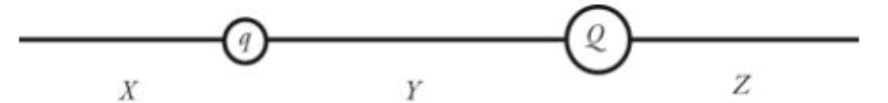
\includegraphics[width=0.5\textwidth]{figures-workshop01/problem-3.png}
    \end{figure}

    \begin{multicols}{5}
    \begin{itemize}
        \item[A)] Only regions $X$ and $Z$
        \item[B)] Only region $X$
        \item[C)] Only region $Y$
        \item[D)] Only region $Z$
        \item[E)] All three regions
    \end{itemize}
    \end{multicols}

    \textbf{Answer:} B

    \item Two very large parallel sheets a distance $d$ apart have their centers directly opposite each other. The sheets carry equal but opposite uniform surface charge densities. A point charge that is placed near the middle of the sheets a distance $d/2$ from each of them feels an electrical force $F$ due to the sheets. If this charge is now moved closer to one of the sheets so that it is a distance $d/4$ from that sheet, what force will feel?

    \begin{multicols}{5}
    \begin{itemize}
        \item[A)] $4F$
        \item[B)] $2F$
        \item[C)] $F$
        \item[D)] $F/2$
        \item[E)] $F/4$
    \end{itemize}
    \end{multicols}

    \textbf{Answer:} C

    \item In the figure, charge $q_1=3.1\,\mu$C is placed at the origin and charge $q_2=-8.7\,\mu$C is placed on the $x$-axis, at $x = -0.20$ m. Where along the $x$-axis can a third charge be placed such that the resultant force on this third charge is zero?

    \begin{figure}[H]
        \centering
        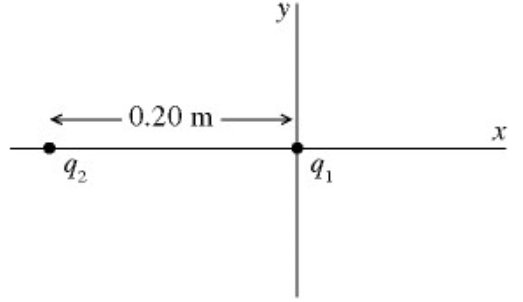
\includegraphics[width=0.4\textwidth,height=0.2\textwidth]{figures-workshop01/problem-5.png}
    \end{figure}

    \textbf{Answer:} 0.30 m

    \item Two small insulating spheres are attached to silk threads and aligned vertically as shown in the figure. These spheres have equal masses of 40 g, and carry charges $q_1$ and $q_2$ of equal magnitude 2.0 $\mu$C but opposite sign. The spheres are brought into the positions shown in the figure, with a vertical separation of 15 cm between them. Note that you cannot neglect gravity. The tension in the lower thread is closest to

    \begin{figure}[H]
        \centering
        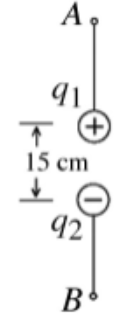
\includegraphics[width=0.08\textwidth]{figures-workshop01/problem-6.png}
    \end{figure}

    \begin{multicols}{5}
    \begin{itemize}
        \item[A)] $1.2$ N
        \item[B)] $1.4$ N
        \item[C)] $1.6$ N
        \item[D)] $1.8$ N
        \item[E)] $2.0$ N
    \end{itemize}
    \end{multicols}

    \textbf{Answer:} A
    
    \item The point charge at the bottom of the figure is $Q=+17$ nC, and the curve is a circular arc. What is the magnitude of the force on the charge $Q$ due to the other point charges shown

    \begin{figure}[H]
        \centering
        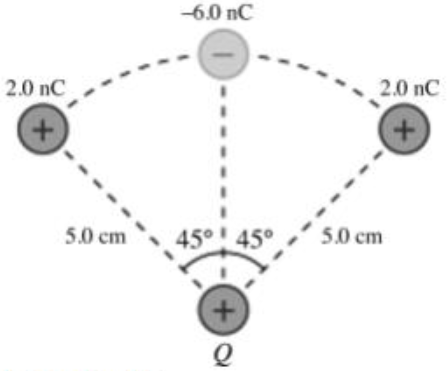
\includegraphics[width=0.3\textwidth]{figures-workshop01/problem-7.png}
    \end{figure}

    \begin{multicols}{5}
    \begin{itemize}
        \item[A)] $1.9\times10^{-4}$ N
        \item[B)] $1.2\times10^{-4}$ N
        \item[C)] $1.6\times10^{-4}$ N
        \item[D)] $2.3\times10^{-4}$ N
    \end{itemize}
    \end{multicols}

    \textbf{Answer:} A

    \item In the figure, a small spherical insulator of mass$ 6.00 \times 10^{-2}$ kg and charge $+0.400 \,\mu$C is hung by a thin wire of negligible mass. A charge of $-0.220\,\mu$C is held 0.290 m away from the sphere and directly to the right of it, so the wire makes an angle $\theta$ with the vertical, as shown. What is the angle $\theta$?

    \begin{figure}[H]
        \centering
        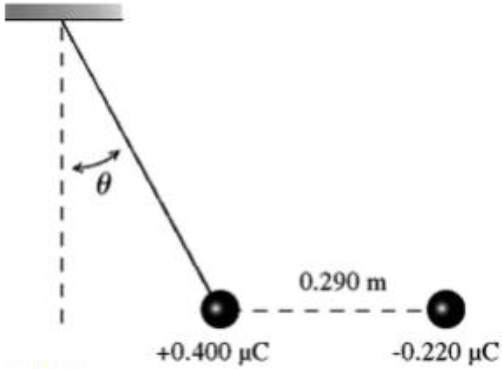
\includegraphics[width=0.32\textwidth]{figures-workshop01/problem-8.png}
    \end{figure}

    \begin{multicols}{5}
    \begin{itemize}
        \item[A)] $0.917^\circ$
        \item[B)] $1.10^\circ$
        \item[C)] $1.30^\circ$
        \item[D)] $1.50^\circ$
        \item[E)] $1.70^\circ$
    \end{itemize}
    \end{multicols}

    \textbf{Answer:} A

    \item A small glass bead has been charged to 8.0 nC. What is the magnitude of the electric field 2.0 cm from the center of the bead?

    \begin{multicols}{5}
    \begin{itemize}
        \item[A)] $1.8\times10^5$ N/C
        \item[B)] $3.6\times10^3$ N/C
        \item[C)] $1.4\times10^{-3}$ N/C
        \item[D)] $3.6\times10^{-5}$ N/C
    \end{itemize}
    \end{multicols}

    \textbf{Answer:} A

    \item A point charge $Q$ of mass 8.50 g hangs from the horizontal ceiling by a light 25.0 cm thread. When a horizontal electric field of magnitude 1750 N/C is turned on, the charge hangs away from the vertical as shown in the figure. The magnitude of $Q$ is closest to

    \begin{figure}[H]
        \centering
        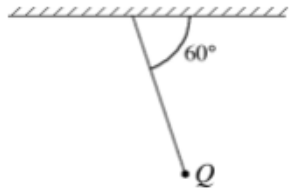
\includegraphics[width=0.22\textwidth]{figures-workshop01/problem-10.png}
    \end{figure}

    \begin{multicols}{5}
    \begin{itemize}
        \item[A)] 27.5 $\mu$C
        \item[B)] 47.6 $\mu$C
        \item[C)] 55.0 $\mu$C
        \item[D)] 3.0 $\mu$C
        \item[E)] 3.5 $\mu$C
    \end{itemize}
    \end{multicols}

    \textbf{Answer:} A

    \item A long, thin rod parallel to the $y$-axis is located at $x = -1.0$ cm and carries a uniform linear charge density of $+1.0$ nC/m. A second long, thin rod parallel to the z-axis is located at $x=+1.0$ cm and carries a uniform linear charge density of $-1.0$ nC/m. What is the net electric field due to these rods at the origin?

    \begin{multicols}{4}
    \begin{itemize}
        \item[A)] $(-3.6\times10^3\text{ N/C})\hat\imath$
        \item[B)] $(1.8\times10^3\text{ N/C})\hat \jmath$
        \item[C)] $(-1.8\times10^3\text{ N/C})\hat k$
        \item[D)] $(3.6\times10^3\text{ N/C})\hat\imath$
        \item[E)] Zero
    \end{itemize}
    \end{multicols}
    

    \textbf{Answer:} D

    \item In the figure, a ring 0.71 m in radius carries a charge of $+580$ nC uniformly distributed over it. A point charge $Q$ is placed at the center of the ring. The electric field is equal to zero at field point $P$, which is on the axis of the ring, and 0.73 m from its center. The point charge $Q$ is closest to

    \begin{figure}[H]
        \centering
        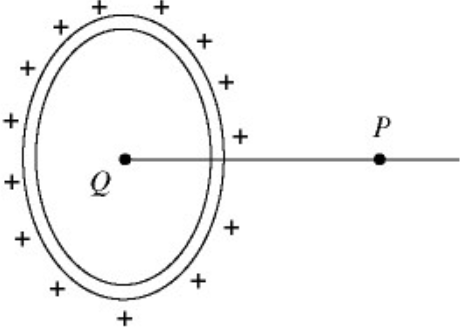
\includegraphics[width=0.28\textwidth]{figures-workshop01/problem-12.png}
    \end{figure}

    \begin{multicols}{5}
    \begin{itemize}
        \item[A)] $-210$ nC
        \item[B)] $-300$ nC
        \item[C)] $-420$ nC
        \item[D)] 210 nC
        \item[E)] 300 nC
    \end{itemize}
    \end{multicols}

    \textbf{Answer:} A

    \item A pair of charged conducting plates produces a uniform field of $12\,000$ N/C, directed to the right, between the plates. The separation of the plates is 40 mm. An electron is projected from plate $A$, directly toward plate $B$, with an initial velocity of $v_0=1.0\times10^7$ m/s, as shown in the figure. The distance of closest approach of the electron to plate $B$ is nearest to

    \begin{figure}[H]
        \centering
        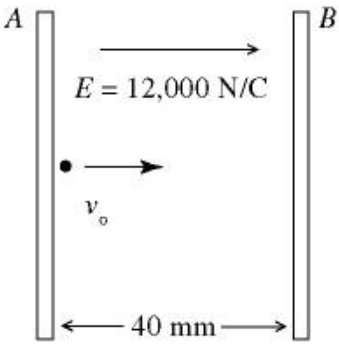
\includegraphics[width=0.22\textwidth]{figures-workshop01/problem-13.png}
    \end{figure}

    \begin{multicols}{5}
    \begin{itemize}
        \item[A)] 16 mm
        \item[B)] 18 mm
        \item[C)] 20 mm
        \item[D)] 22 mm
        \item[E)] 24 mm
    \end{itemize}
    \end{multicols}

    \textbf{Answer:} A

    \item In the figure, a proton is projected horizontally midway between two parallel plates that are separated by 0.50 cm. The electrical field due to the plates has magnitude $610\,000$ N/C between the plates away from the edges. If the plates are 5.60 cm long, find the minimum speed of the proton if it just misses the lower plate as it emerges from the field.

    \begin{figure}[H]
        \centering
        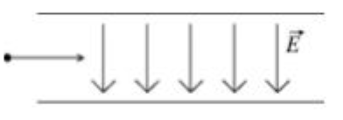
\includegraphics[width=0.32\textwidth]{figures-workshop01/problem-14.png}
    \end{figure}

    \textbf{Answer:} $6.06\times10^6$ m/s

    \item An electric dipole is made of two charges of equal magnitudes and opposite signs. The positive charge, $q = 1.0\,\mu$C, is located at the point $(x, y, z) = (0.00 \text{ cm}, 1.0 \text{ cm}, 0.00 \text{ cm})$, while the negative charge is located at the point $(x, y, z) = (0.00 \text{ cm}, -1.0 \text{ cm}, 0.00 \text{ cm})$. How much work will be done by an electric field $\vec{E}= (3.0 \times 10^6 \text{ N/C})\hat\imath$ to bring the dipole to its stable equilibrium position?

    \begin{multicols}{5}
    \begin{itemize}
        \item[A)] 60 mJ
        \item[B)] 30 mJ
        \item[C)] 0
        \item[D)] 20 mJ
        \item[E)] 120 mJ
    \end{itemize}
    \end{multicols}

    \textbf{Answer:} A

    \item An initially-stationary electric dipole of dipole moment $\vec{p}=(5.00 \times 10^{-10} \text{ C} \cdot \text{m})\hat\imath$ placed in an electric field $\vec{E}= (2.00 \times 10^6 \text{ N/C})\hat{\imath} + (2.00 \times 10^6 \text{ N/C})\hat{\jmath}$ . What is the magnitude of the maximum torque that the electric field exerts on the dipole?

    \begin{multicols}{5}
    \begin{itemize}
        \item[A)] $2.0\times10^{-3}\text{ N}\cdot\text{m}$ 
        \item[B)] $1.4\times10^{-3}\text{ N}\cdot\text{m}$ 
        \item[C)] $2.8\times10^{-3}\text{ N}\cdot\text{m}$ 
        \item[D)] 0.0 $\text{N}\cdot\text{m}$ 
        \item[E)] $1.0\times10^{-3}\text{ N}\cdot\text{m}$ 
    \end{itemize}
    \end{multicols}

    \textbf{Answer:} E

    \item $\color{red}{\star}$ A hemispherical shell has radius $R$ and uniform surface charge density $\sigma$ (see figure). Find the electric field at a point on the symmetry axis, at position $z$ relative to the center, for any $z$ value from $-\infty$ to $\infty$.

    \begin{figure}[H]
        \centering
        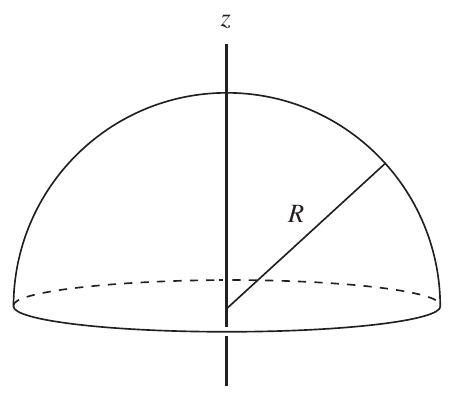
\includegraphics[width=0.22\textwidth]{figures-workshop01/problem-17.png}
    \end{figure}

    \item $\color{red}{\star}$ A charge $2q$ is at the origin, and a charge $-q$ is at $x=a$ on the $x$-axis.

    \begin{itemize}
        \item[a)] Find the point on the $x$-axis where the electric field is zero.
        \item[b)] Consider the vertical line passing through the charge $-q$, that is, the line given by $x=a$. Locate, at least approximately, a point on this line where the electric field is parallel to the $x$-axis.
    \end{itemize}

    \item $\color{red}{\star}$ A half-infinite line has linear charge density $\lambda$. Find the electric field at a point that is “even” with the end, a distance $l$ from it, as shown in figure. You should find that the field always points up at a $45^\circ$ angle, independent of $l$.

    \begin{figure}[H]
        \centering
        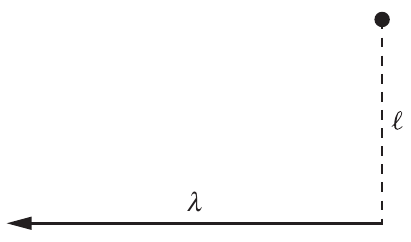
\includegraphics[width=0.22\textwidth]{figures-workshop01/problem-18.png}
    \end{figure}

    \item A ring with radius $R$ has uniform positive charge density $\lambda$. A particle with positive charge $q$ and mass $m$ is initially located at the center of the ring and is then given a tiny kick. If it is constrained to move in the plane of the ring, show that it undergoes simple harmonic motion (for small oscillations), and find the frequency. \textit{Hint}: Find the potential energy of the particle when it is at a (small) radius, $r$, by integrating over the ring, and then take the negative derivative to find the force. You will need to use the law of cosines and also the Taylor series $1/\sqrt{1+\epsilon}\approx1-\epsilon/2+3\epsilon^2/8$.

    \item A charge $Q$ is uniformly spread over one surface of a very large nonconducting square elastic sheet having sides of length $d$. At a point $P$ that is 1.25 cm outside the sheet, the magnitude of the electric field due to the sheet is $E$. If the sheet is now stretched so that its sides have length $2d$, what is the magnitude of the electric field at $P$?

    \begin{multicols}{5}
    \begin{itemize}
        \item[A)] $4E$
        \item[B)] $2E$
        \item[C)] $E$
        \item[D)] $E/2$
        \item[E)] $E/4$
    \end{itemize}
    \end{multicols}

    \textbf{Answer:} E

    \item An uncharged conductor has a hollow cavity inside of it. Within this cavity there is a charge of $+10\,\mu$C that does not touch the conductor. There are no other charges in the vicinity. Which statement about this conductor is true? (There may be more than one correct choice)
    
    \begin{itemize}
        \item[A)] The inner surface of the conductor carries a charge of $-10\,\mu$C and its outer surface carries no excess charge.
        \item[B)] The inner and outer surfaces of the conductor each contain charges of $-5\,\mu$C.
        \item[C)] The net electric field within the material of the conductor points away from the $+10\,\mu$C charge.
        \item[D)] The outer surface of the conductor contains $+10\,\mu$C of charge and the inner surface contains $-10\,\mu$C.
        \item[E)] Both surfaces of the conductor carry no excess charge because the conductor is uncharged.
    \end{itemize}

    \textbf{Answer:} D

    \item A cone is resting on a tabletop as shown in the figure with its face horizontal. A uniform electric field of magnitude $4\,550$ N/C points vertically upward. How much electric flux passes through the sloping side surface area of the cone?

    \begin{figure}[H]
        \centering
        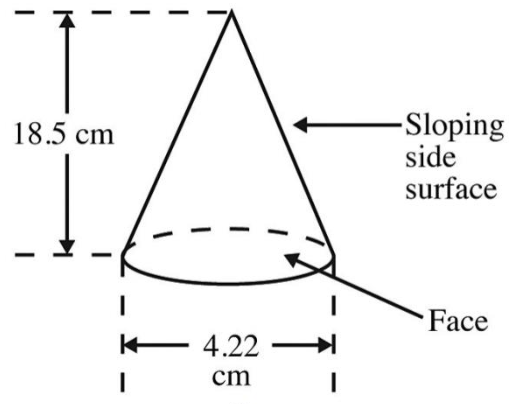
\includegraphics[width=0.32\textwidth]{figures-workshop01/problem-23.png}
    \end{figure}

    \textbf{Answer:} 6.36 N$\cdot$m$^2$/C

    \item The cross-section of a long coaxial cable is shown in the figure, with radii as given. The linear charge density on the inner conductor is $-30$ nC/m and the linear charge density on the outer conductor is $-70$ nC/m. The inner and outer cylindrical surfaces are respectively denoted by $A$, $B$, $C$, and $D$, as shown. The radial component of the electric field at a point that 34 mm from the axis is closest to

    \begin{figure}[H]
        \centering
        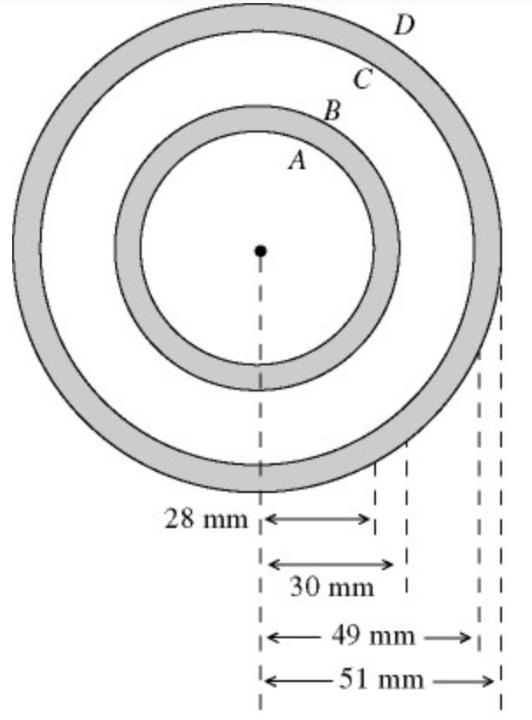
\includegraphics[width=0.3\textwidth]{figures-workshop01/problem-24.png}
    \end{figure}

    \begin{multicols}{5}
    \begin{itemize}
        \item[A)] $-16\,000$ N/C
        \item[B)] $+16\,000$ N/C
        \item[C)] $-37\,000$ N/C
        \item[D)] $+37\,000$ N/C
        \item[E)] zero
    \end{itemize}
    \end{multicols}

    \textbf{Answer:} A

    \item As shown in the figure, a square insulating slab 5.0 mm thick measuring $2.0\text{ mm}\times2.00\text{ mm}$ has a charge of $8.00\times10^{-11}$ C distributed uniformly throughout its volume. Use Gauss's law to determine the electric field at point $P$, which is located within the slab beneath its center, 1.0 mm from one of the faces.

    \begin{figure}[H]
        \centering
        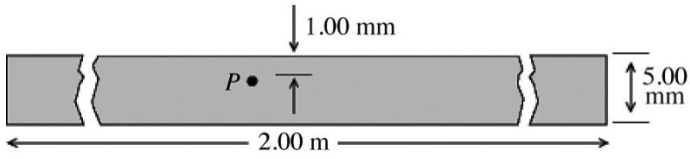
\includegraphics[width=0.4\textwidth]{figures-workshop01/problem-25.png}
    \end{figure}

    \begin{multicols}{5}
    \begin{itemize}
        \item[A)] $0.68$ N/C
        \item[B)] $14$ N/C
        \item[C)] $23$ N/C
        \item[D)] $34$ N/C
        \item[E)] $57$ N/C
    \end{itemize}
    \end{multicols}

    \textbf{Answer:} A

    \item Two extremely large nonconducting horizontal sheets each carry uniform charge density on the surfaces facing each other. The upper sheet carries $+5.00\,\mu$C/m$^2$. The electric field midway between the sheets is $4.25\times10^5$ N/C pointing downward. What is the surface charge density on the lower sheet?

    \textbf{Answer:} $-2.52\,\mu$C/m$^2$

    \item Consider two closely spaced and oppositely charged parallel metal plates. The plates are square with sides of length $L$ and carry charges $Q$ and $-Q$ on their facing surfaces. What is the magnitude of the electric field in the region between the plates?

\begin{multicols}{5}
    \begin{itemize}
        \item[A)] $E = \dfrac{Q}{\epsilon_0L^2}$
        \item[B)] $E = \dfrac{2Q}{\epsilon_0L^2}$.
        \item[C)] $E=0$.
        \item[D)] $E = \dfrac{4Q}{\epsilon_0L^2}$.
        \item[E)] $E = \dfrac{Q}{2\epsilon_0L^2}$.
    \end{itemize}
\end{multicols}

\textbf{Answer:} A

\item $\color{red}{\star}$ Two point charges $q$ are located at positions $x = \pm l$. At points
close to the origin on the $x$-axis, find $E_x$ . At points close to the
origin on the $y$-axis, find $E_y$. Make suitable approximations
with $x<<l$ and $y<<l$.

\item $\color{red}{\star}$ Consider a small cylinder centered at the origin, with its axis
along the $x$-axis. The radius is $r_0$ and the length is $2x_0$. Using
your results from the previous problem, verify that there is zero flux through
the cylinder, as required by Gauss’s law.
    
\item $\color{red}{\star}$ Consider a large flat horizontal sheet with thickness $x$ and volume
charge density $\rho$. This sheet is tangent to a sphere with radius $R$
and volume charge density $\rho_0$, as shown in figure. Let $A$ be the
point of tangency, and let $B$ be the point opposite to $A$ on the top
side of the sheet. Show that the net upward electric field (from
the sphere plus the sheet) at $B$ is larger than at $A$ if $\rho>(2/3)\rho_0$
(assume $x<<R$).

    \begin{figure}[H]
        \centering
        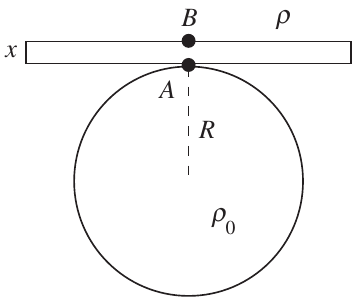
\includegraphics[width=0.28\textwidth]{figures-workshop01/problem-30.png}
    \end{figure}

    \item $\color{red}{\star}$ A charge $Q$ is distributed uniformly around a thin ring of radius $b$ that lies in the $xy$ plane with its center at the origin. Locate the
point on the positive $z$-axis where the electric field is
strongest.

\item $\color{red}{\star\star}$ $N$ point charges, each with charge $Q/N$, are evenly distributed
around a circle of radius $R$. What is the electric field at the location of one of the charges, due to all the others? (You can leave
your answer in the form of a sum.) In the $N\rightarrow\infty$ limit, is the
field infinite or finite? In the $N\rightarrow\infty$ limit, is the force on one of
the charges infinite or finite?

\item Suppose you have two negative point charges. As you move them farther and farther apart, the potential energy of this system relative to infinity

\begin{multicols}{5}
    \begin{itemize}
        \item[A)] increases
        \item[B)] decreases
        \item[C)] stays the same
    \end{itemize}
\end{multicols}

\textbf{Answer:} B

\item A conducting sphere contains positive charge distributed uniformly over its surface. Which statements about the potential due to this sphere are true? All potentials are measured relative to infinity. (There may be more than one correct choice.)

\begin{itemize}
    \item[A)] The potential is lowest, but not zero, at the center of the sphere.
    \item[B)] The potential at the center of the sphere is zero.
    \item[C)] The potential at the center of the sphere is the same as the potential at the surface.
    \item[D)] The potential at the surface is higher than the potential at the center.
    \item[E)] The potential at the center is the same as the potential at infinity.
\end{itemize}

\textbf{Answer:} C

\item A negative charge is moved from point $A$ to point $B$ along an equipotential surface. Which of the following statements must be true for this case?

\begin{itemize}
    \item[A)] The negative charge performs work in moving from point $A$ to point $B$.

\item[B)] Work is required to move the negative charge from point $A$ to point $B$.

\item[C)] No work is required to move the negative charge from point $A$ to point $B$.

\item[D)] The work done on the charge depends on the distance between $A$ and $B$.

\item[E)] Work is done in moving the negative charge from point $A$ to point $B$.
\end{itemize}

\textbf{Answer:} C

\item The potential as a function of position $x$ is shown in the graph in the figure. Which statement about the electric field is true?

\begin{figure}[H]
        \centering
        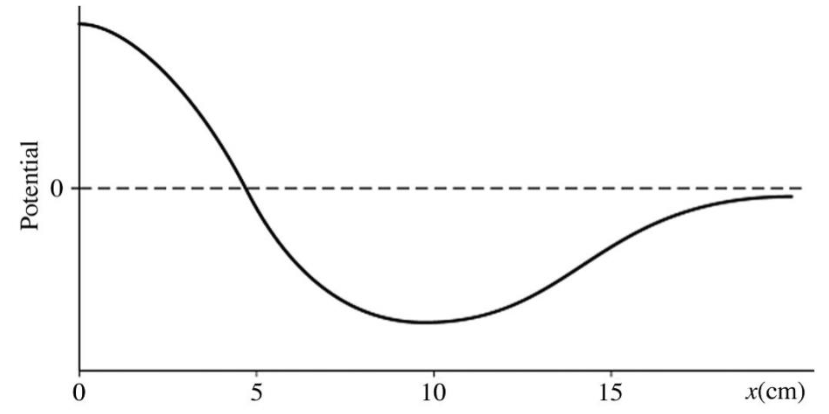
\includegraphics[width=0.38\textwidth]{figures-workshop01/problem-36.png}
    \end{figure}

\begin{itemize}
    \item[A)] The electric field is zero at $x = 0$, its magnitude is at a maximum at $x = 5$ cm, and the field is directed to the right there.

\item[B)] The electric field is zero at $x = 5$ cm, its magnitude is at a maximum at $x = 0$, and the field is directed to the right there.

\item[C)] The electric field is zero at $x = 0$, its magnitude is at a maximum at $x = 15$ cm, and the field is directed to the left there.

\item[D)] The electric field is zero at $x = 10$ cm, its magnitude is at a maximum at $x = 5$ cm, and the field is directed to the left there.
\end{itemize}

\textbf{Answer:} A

\item Two positive point charges $+4.00\,\mu$C and $+2.00\,\mu$C are placed at the opposite corners of a rectangle as shown in the figure.

\begin{figure}[H]
        \centering
        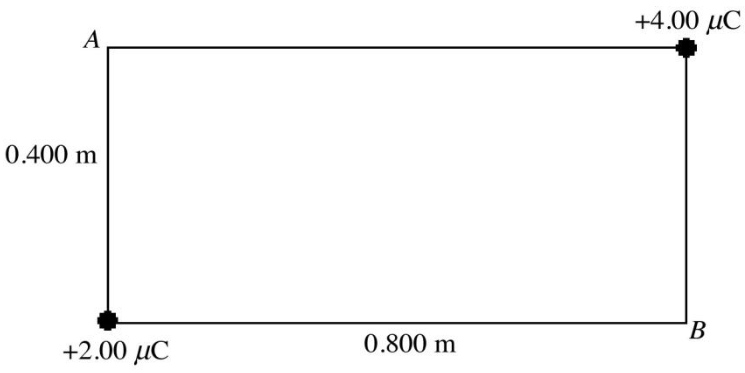
\includegraphics[width=0.38\textwidth]{figures-workshop01/problem-37.png}
    \end{figure}

\begin{itemize}
    \item[a)] What is the potential at point $A$ (relative to infinity) due to these charges?
    \item[b)] What is the potential at point $B$ (relative to infinity) due to these charges?
\end{itemize}

%\textbf{Answers:} (a) $+8.99 \times 104$ V, (b) $1.12 \times 105$ V

\item The figure shows two arcs of a circle on which charges $+Q$ and $-Q$ have been spread uniformly. What is the value of the electric potential at the center of the circle?

\begin{figure}[H]
        \centering
        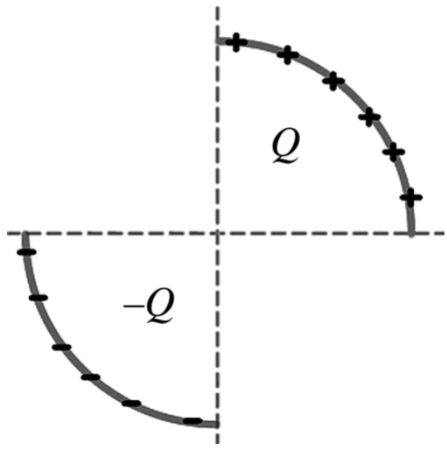
\includegraphics[width=0.28\textwidth]{figures-workshop01/problem-38.png}
    \end{figure}

\textbf{Answer:} Zero

\item Two large conducting parallel plates $A$ and $B$ are separated by 2.4 m. A uniform field of $1\,500$ V/m, in the positive $x$-direction, is produced by charges on the plates. The center plane at $x=0.00$ m is an equipotential surface on which $V=0$. An electron is projected from $x=0.00$ m, with an initial velocity of $1,0\times10^7$ m/s perpendicular to the plates in the positive $x$-direction, as shown in the figure. What is the kinetic energy of the electron as it reaches plate $A$?

\begin{figure}[H]
        \centering
        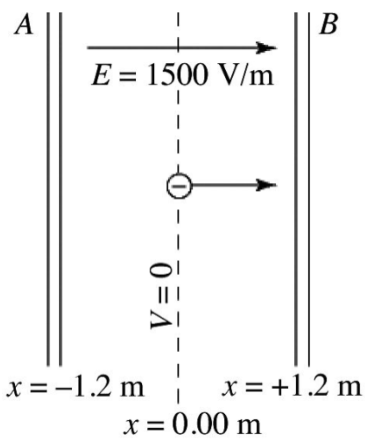
\includegraphics[width=0.28\textwidth]{figures-workshop01/problem-39.png}
    \end{figure}

\begin{multicols}{5}
    \begin{itemize}
        \item[A)] $+2.4\times10^{-16}$ J
        \item[B)] $+3.3\times10^{-16}$ J
        \item[C)] $-2.4\times10^{-16}$ J
        \item[D)] $-2.9\times10^{-16}$ J
        \item[E)] $-3.3\times10^{-16}$ J
    \end{itemize}
\end{multicols}

\textbf{Answer:} B

\item A very long, solid cylinder, with radius $R$, has positive charge distributed uniformly, with charge per unit volume $\rho$.

\begin{itemize}
    \item[a)] Obtain the expression for the electric field inside the volume at a distance $r$ from the axis of the cylinder in terms of the charge density $r$.
    \item[b)] What is the electric field at a point outside the volume in terms of the charge per unit length $l$ on the cylinder?
    \item[c)] Compare your answers to parts (a) and (b) for $r = R$. 
    \item[d)] Plot a graph of the magnitude of the electric field as a function of $r$, from $r = 0$ to $r = 3R$.
\end{itemize}

\newpage

\section*{Answers}

\begin{multicols}{4}
    \begin{table}[H]
\begin{tabular}{|c|c|}
\hline
\textbf{1}  & C \\ \hline
\textbf{2}  & C \\ \hline
\textbf{3}  & B \\ \hline
\textbf{4}  & C \\ \hline
\textbf{5}  & 0.30 \text{m}\\ \hline
\textbf{6}  & A \\ \hline
\textbf{7}  & A \\ \hline
\textbf{8}  & A \\ \hline
\textbf{9}  & A \\ \hline
\textbf{10} & A \\ \hline
\end{tabular}
\end{table}

\begin{table}[H]
\begin{tabular}{|c|c|}
\hline
\textbf{11}  & D \\ \hline
\textbf{12}  & A \\ \hline
\textbf{13}  & A \\ \hline
\textbf{14}  & $6.06\times10^6\,\text{m}/\text{s}$ \\ \hline
\textbf{15}  & A \\ \hline
\textbf{16}  & E \\ \hline
\textbf{17}  &  \\ \hline
\textbf{18}  &  \\ \hline
\textbf{19}  &  \\ \hline
\textbf{20} &  \\ \hline
\end{tabular}
\end{table}

\begin{table}[H]
\begin{tabular}{|c|c|}
\hline
\textbf{21}  & E \\ \hline
\textbf{22}  & D \\ \hline
\textbf{23}  & $6.36\,\text{N}\cdot\text{m}^2/\text{C}$ \\ \hline
\textbf{24}  & A \\ \hline
\textbf{25}  & A \\ \hline
\textbf{26}  & $-2.52\,\mu\text{C}/\text{m}^2$ \\ \hline
\textbf{27}  & A \\ \hline
\textbf{28}  &  \\ \hline
\textbf{29}  &  \\ \hline
\textbf{30} &  \\ \hline
\end{tabular}
\end{table}

\begin{table}[H]
\begin{tabular}{|c|c|}
\hline
\textbf{31}  &  \\ \hline
\textbf{32}  &  \\ \hline
\textbf{33}  & B \\ \hline
\textbf{34}  & C \\ \hline
\textbf{35}  & C \\ \hline
\textbf{36}  & A \\ \hline
\textbf{37}  &  \\ \hline
\textbf{38}  & Zero \\ \hline
\textbf{39}  & B \\ \hline
\textbf{40} &  \\ \hline
\end{tabular}
\end{table}
\end{multicols}

\end{enumerate}




\end{document}